\section{Hyperparameters for Soft Actor Critic Training}
\subsection{}
% SAC training workflow
  % \cite{haarnoja2018soft}
  \begin{figure}[H]
      \centering
      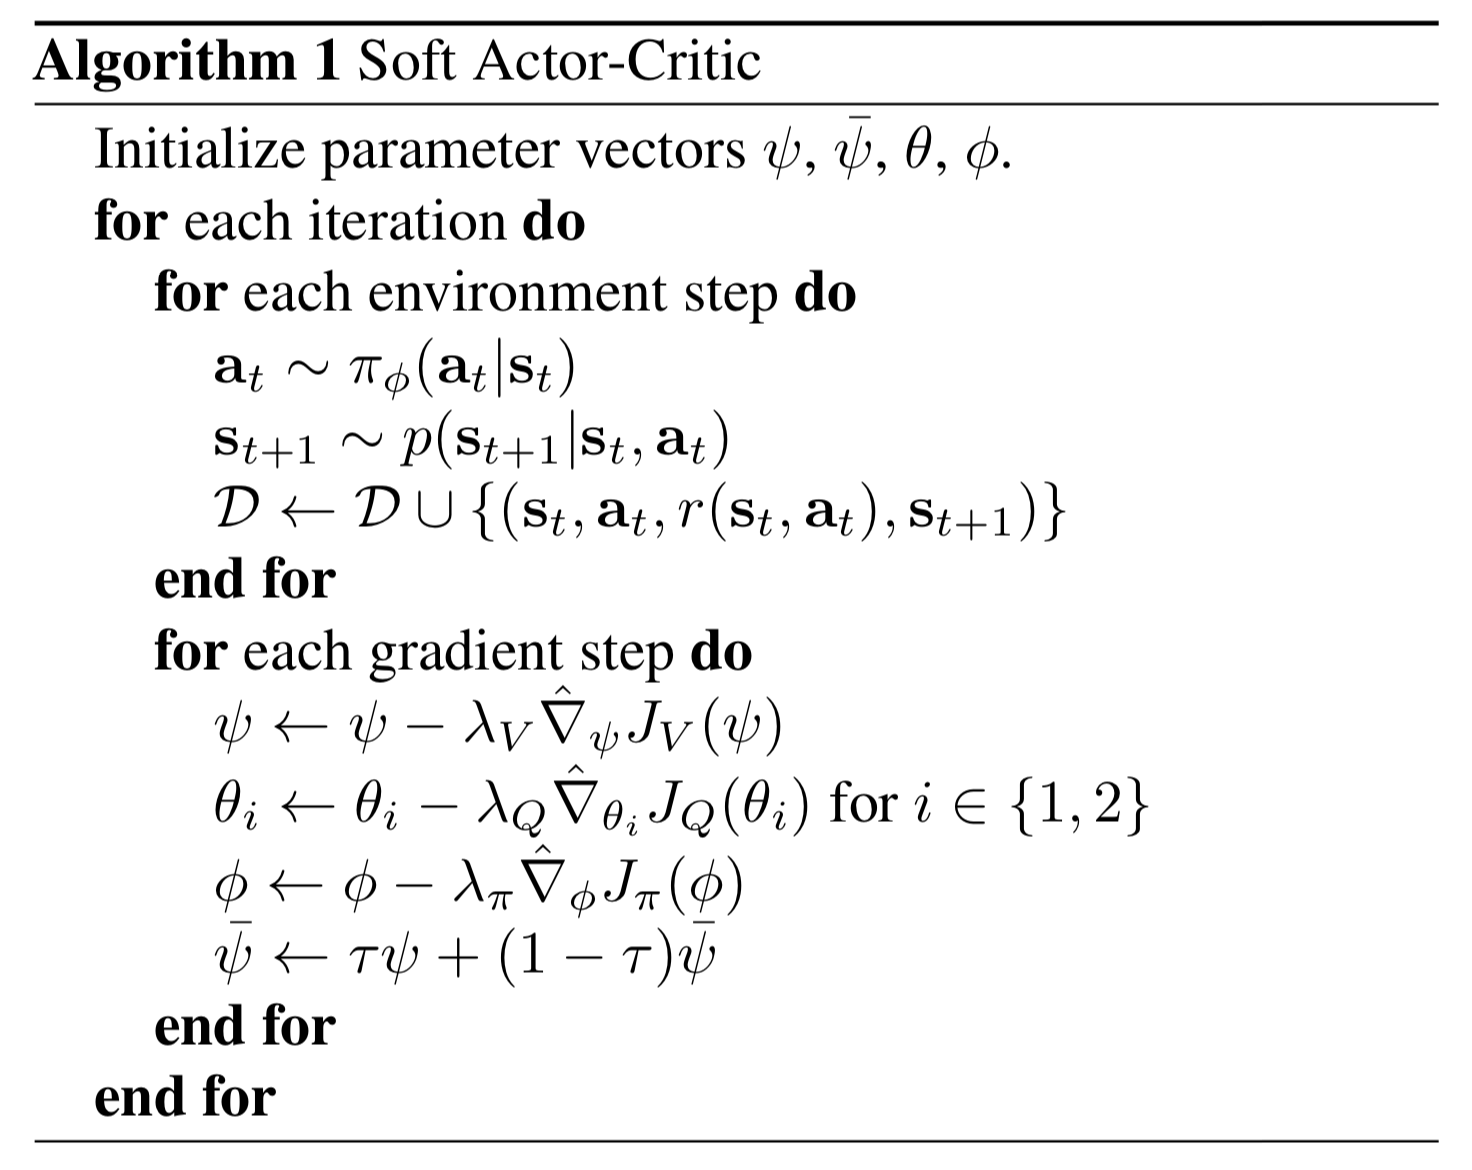
\includegraphics[width=1\textwidth / 2]{figures/external/sac_algorithm.png}
      \caption{Soft Actor Critic algorithm as seen in \cite{haarnoja2018soft}}
      \label{fig:sac_algorithm}
  \end{figure}

% batch training
% hidden layer size 256
% epochs 3000

% timesteps per training loop 1000
% param update per training loop 1000
% batch size 256
% replay_buffer_size=int(1E6),

% layer_size=256,
%     replay_buffer_size=int(1E6),
%     algorithm_kwargs=dict(
%         num_epochs=3000,
%         num_eval_steps_per_epoch=5000, % this is for evaluation
%         num_trains_per_train_loop=1000,
%         num_expl_steps_per_train_loop=1000,
%           min_num_steps_before_training=1000,
%           max_path_length=1000,
%         batch_size=256,
%     ),
%     trainer_kwargs=dict(
%         discount=0.99,
%         soft_target_tau=5e-3,
%         target_update_period=1,
%         policy_lr=3E-4,
%         qf_lr=3E-4,
%         reward_scale=1,
%         use_automatic_entropy_tuning=True,
%     ),
